%!TEX root = ../thesis.tex
%*******************************************************************************
%****************************** Second Chapter *********************************
%*******************************************************************************

\chapter{Methodology}

The core task of the project is to investigate the prediction accuracy of directional branch predictors
under WSC workload. To achieve this, WSC branch traces that fit real-world WSC load scenarios are 
needed, and a sufficiently efficient and well-accepted simulator is required to make the result 
convincing, not to mention a high-performance platform to provide the computing resources.

This section demonstrates where and how the the experiment are implemented.

\ifpdf
    \graphicspath{{Chapter2/Figs/Raster/}{Chapter2/Figs/PDF/}{Chapter2/Figs/}}
\else
    \graphicspath{{Chapter2/Figs/Vector/}{Chapter2/Figs/}}
\fi

\section{Simulation infrastructure}

\subsection{5th Branch Prediction Championship (CBP-5) Kit}

CBP-5 \cite{noauthor_championship_nodate} is a conditional branch predictor simulator provided by Branch Prediction Championship, a competition organised by \textit{The Journal of Instruction-Level Parallelism}. Since the first competition was held in 2004, CBP has gradually become a widely accepted branch predictor simulator. \par\hspace*{\fill}\par

There are several reasons why CBP-5 is very well suited to this project. Firstly, it is speedy. Unlike 
Gem5, QEMU and other whole-chip simulation tools, CBP-5 focuses on the directional branch 
predictors' simulation and is implemented in C++, thus can simulates far faster than Gem5 and QEMU. Secondly, its simplicity reduces potential hurdles when being applied to other trace formats (e.g. Google Workload Traces). The smooth learning curve also makes it more suitable for this time-critical project. Finally, there are useful branch instruction traces (223 training traces) and SOTA predictors (winner submission of the competition) attached to this simulator kit and can help streamline project workload.

\subsubsection{CBP-5 traces}
223 traces are given in the CBP-5 kit and separated into four catagories: 19 long mobile traces, 61 short mobile traces, 4 long server traces and 139 short server traces. Long traces have 1 billion instructions and shot traces have 100 million instructions. In this project we combine all 80 mobile traces as CBP-5 \textit{mobile} trace set, and all 143 server traces as CBP-5 \textit{server} trace set.

\subsubsection{CBP-5 predictors}
11 prize-winning predictors are given in the CBP-5 kit, including SOTA \textbf{TAGE-SC-L}\cite{seznec_tage-sc-l_2016} (8KB \& 64KB), \textbf{MTAGE+SC}\cite{seznec_exploring_2016} (Unlimited size),\textbf{ Multiperspective Perceptron Predictor}\cite{jimenez_multiperspective_2016} (8KB, 64KB \& Unlimited), \textbf{Multiperspective Perceptron Predictor with TAGE}\cite{jimenez_multiperspective_2016-1} (8KB, 64KB \& Unlimited) and \textbf{Dynamically Sized TAGE}\cite{pruett_dynamically_2016} (8KB \& 64KB). All predictors are simulated but the discussion on predictors is focused on TAGE-SC-L, MTAGE-SC and Multiperspective Perceptron with TAGE.

\subsubsection{CBP-5 trace format: BT9}
CBP-5 uses \textit{Branch Trace version 9} (BT9) as its input file format. A complete branch instruction trace is translated into the a flow control graph (e.g. Figure~\ref{fig:branch graph}) and its node table, edge table and edge sequence are stored in a BT9 file, therefore being a space-saving format.

\begin{figure}[h!] 
\centering    
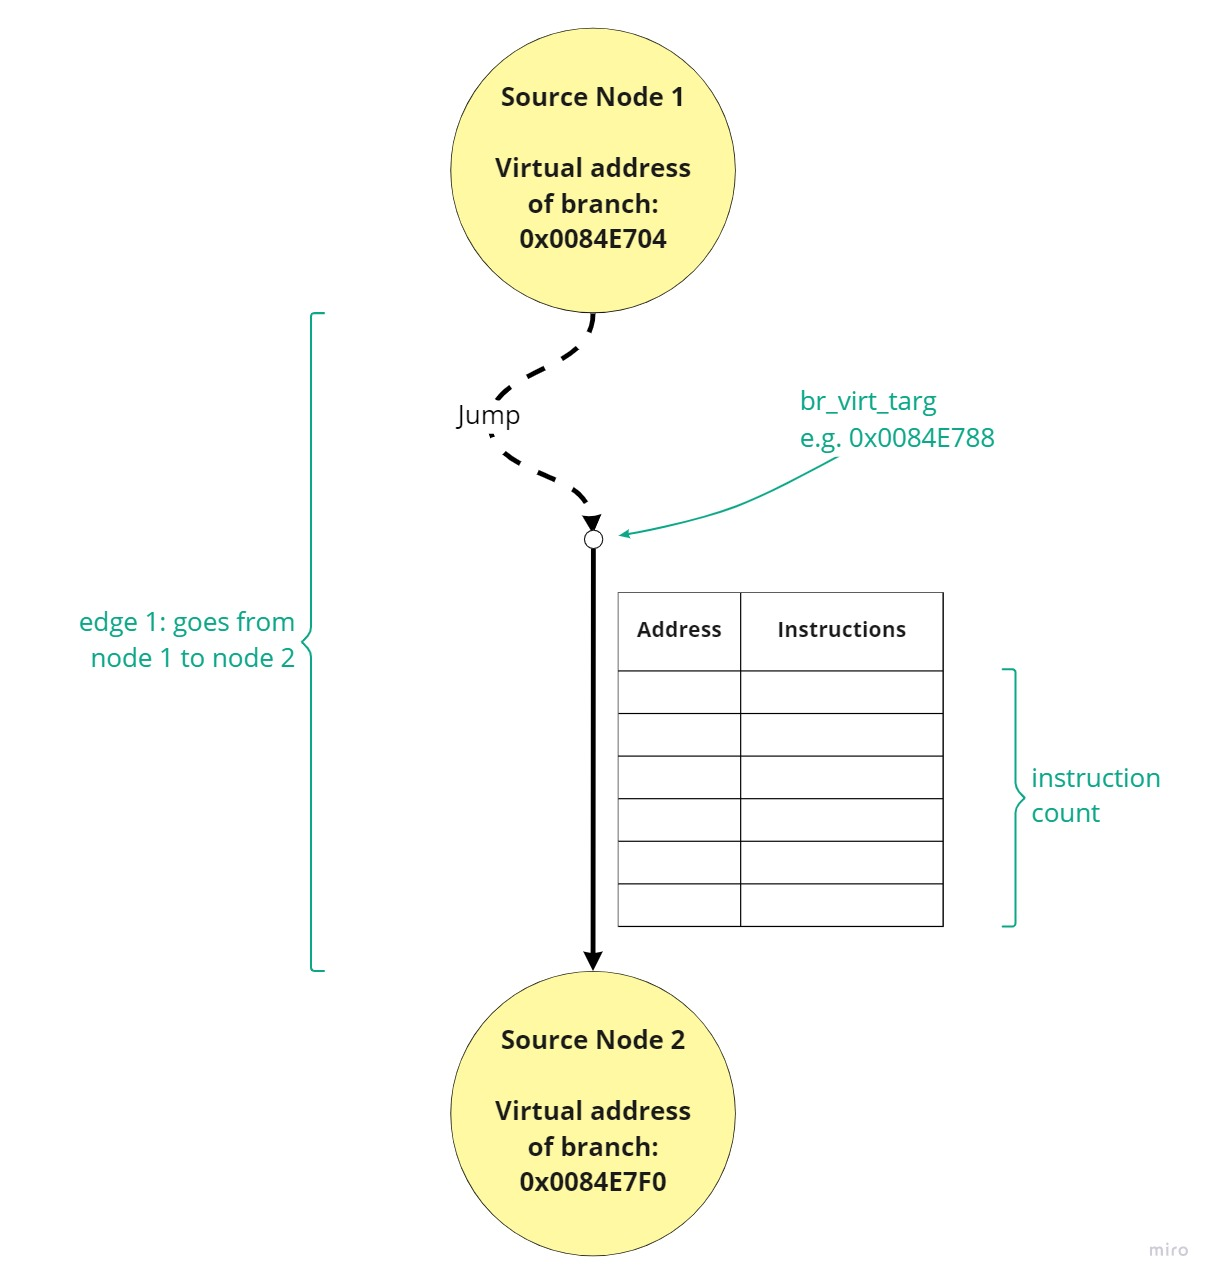
\includegraphics[width=0.5\textwidth]{Chapter2/branch graph.jpg}
\caption{\centering BT9 format example: control flow graph}
\label{fig:branch graph}
\end{figure} 


\subsection{Google workload traces}
Released May 2022, the Google Workload Traces\cite{noauthor_google_nodate} project is driven by the rapid growth of warehouse-scale computers (WSCs) in today's computing market and hopes to improve research in the WSC architecture by sharing real WSC workload data. The traces are captured from Google datacentre using \textit{DynamoRIO}'s \textit{drmemtrace}, including instruction and memory address traces (.memtrace.gz) as well as branch traces (branch\_trace.<tid>.csv.gz). Each representing a unique WSC application, there four trace folders named \textit{delta}, \textit{whiskey}, \textit{charlie} and \textit{merced}. All traces inside a folder are captured in a single launch thus sharing virtual address space.\par\hspace*{\fill}\par

As the first published WSC traces, Google workload traces fit well with this project by offering a domain 
different from all traditional benchmarks. At the stage the focus is on the branch traces.


\subsection{Computing platform}

The simulation is power by a HUAWEI server equipping two Intel(R) Xeon(R) Gold 6161 CPUs and 
supporting a maximum of 88 threads. Computing resource is accessed by SSH, and a Docker container 
is created on the server to provide a safe working environment. All simulation data is analysed by \textit{numpy} and plotted by \textit{matplotlib}. 



\section{BT9 Format conversion}
\label{BT9 Converson}

This section stems from the mismatch between the CBP-5 and WSC branch trace formats; CBP-5 uses the BT9 format, while WSC traces are captured by DynamoRIO and therefore use the DynamoRIO format. There are two potential solutions to the mismatch, either designing a program that converts Google WSC traces into BT9 format or modifying the frontend part of CBP-5. The former option is taken in this project, beacuse designing a program that only formats the WSC trace would make the risk more manageable than modifying the simulator with thousands of lines of code. Besides, modified CBP-5 may reduce the acceptance of the results. \par\hspace*{\fill}\par

This is one of the core objectives of the project and takes the major project period. Since a WSC trace is structured as a sequential branch instruction list while a BT9 file is stored as node table (unique branches), edge table and edge sequence (abbreviated branch instructions), the foundamental idea of conversion is simple: read branch instruction one by one trace file, update the node table and edge table, and then append the interpreted edge into edge sequence. \par\hspace*{\fill}\par

However, because of the mismatched information, some unexpected problems were encountered during the conversion leading to a one-week delay.


\subsubsection{Behaviour, size and instruction count}
Though the behaviour information is expected in BT9 format, it is not used in the predictor. Thus we block the behaviour entry in BT9. \par\hspace*{\fill}\par

Instruction count refers to the number of non-branch instructions executed between two branch instructions. Whatever instruction size is used in the calculation, some instruction count are fractions or negative numbers. The invalid instruction count implies that in contrast to the fixed-size instructions in the CBP-5 traces, instructions in Google WSC traces have various sizes (and is presumed to be x86\_64 instruction set)

\subsubsection{Branch type conversion}

The classification of branch types in two formats are different. In BT9, each branch must take a label from each of the following classes:

\begin{description}[itemsep= 0pt,topsep = 0pt, partopsep=4 pt, leftmargin= 32 pt,labelindent=32pt]
\item[Type] \qquad\qquad\qquad Return, Jump, Call
\item[Directness] \qquad\qquad DIRECT, INDIRECT
\item[Conditionality] \qquad CONDITIONAL, UNCONDITIONAL
\end{description}

\hspace*{\fill}\par
However in Google WSC traces, branches are categorised into eight types, as shown in the first column of Table~\ref{table:branch type}. Obviously, the conversion cannot be done directly, and three problems are listed below.

\begin{enumerate}[itemsep= 0pt,topsep = 0pt, partopsep=4 pt, leftmargin= 32 pt]
\item No Google branch types are specified the Conditionality except \textit{conditional jump}

Based on an observation that all branches in Google WSC traces are 100\% taken except \textit{conditional jump}, it is assumed that all other types are unconditional.


\item The \textit{interrupt} and \textit{context switch} do not correspond to any of the BT9 label. \label{interrupt}

This problem indeed exists and cannot be address directly. However, noting that only a tiny fraction of branch instructions are \textit{interrupt} or \textit{context switch} (verified in Section~\ref{frantion of interrupt}), they are ignored in this project by being converted into JMP+DIR+UND, a common and undirectional type that won't affect conditional branch predictors. 

\item The \textit{conditional jump} has no clear Directness

Because the project studies the condition branch predictor only (i.e. predict taken or not-taken), the directness does not affect the simulation results. \textit{conditional jump} interpreted as DIRECT branch because direct branches are the majority of all branches.

\end{enumerate}



\begin{table}
\centering
\begin{tabular}{c c c}
\toprule{\LARGE}
Google WSC type & BT9 type & \textit{problem encountered} \\ 
\cmidrule{1-3}

\textit{direct call}         &   CALL+DIR+UCD    &1\\
\textit{indirect call}       &   CALL+IND+UCD    &1\\
\textit{direct jump}         &   JMP+DIR+UCD     &1\\
\textit{indirect jump}       &   JMP+IND+UCD     &1\\
\textit{conditional jump}    &   JMP+DIR+CND     &3\\
\textit{return}              &   RET+IND+UCD     &1\\
\textit{interrupt}           &   JMP+DIR+UCD     &2\\
\textit{context switch}      &   JMP+DIR+UCD     &2\\

\bottomrule
\end{tabular}
\caption{\centering \small Branch type conversion result}
\label{table:branch type}

\end{table} % branch type table







\nomenclature[z-WSC]{WSC}{Warehouse-Scale Computer}
\nomenclature[z-BT9]{BT9}{Branch Trace version 9, a trace format applied by CBP-5}
\nomenclature[z-MPKI]{MPKI}{Misprediction Pre 1K Instructions}
\nomenclature[z-HTPB]{HTPB}{Hard To Predict Branch}
\nomenclature[z-UDUB]{UDUB}{UniDirectional Unique Branch}
\nomenclature[z-TAGE]{TAGE}{TAgged GEometric history length branch prediction}


\nomenclature[z-PHT]{PHT}{Pattern History Table}
\nomenclature[z-ETPB]{ETPB}{Easy To Predict Branch}
\nomenclature[z-UB]{UB}{Unique Cranch}
\nomenclature[z-PC]{PC}{Program Counter}
\nomenclature[z-PPM]{PPM}{Prediction by Partial Matching}
\nomenclature[z-MPP]{MPP}{Multiperspective Perceptron Predictor}
\nomenclature[z-DS-TAGE]{DS-TAGE}{Dynamically Sized TAGE}

\nomenclature[z-MPP]{MPP-TAGE}{Multiperspective Perceptron Predictor with TAGE}


\nomenclature[x-a]{\textit{Set of trace / trace set}}{
There are six sets of traces: CBP-5 \textit{mobile}, \textit{server}, Google WSC \textit{delta}, \textit{whiskey}, \textit{charlie}, \textit{merced}. Set is the basic unit for the simulation and calculation in the project. For WSC, set is also the maximum range in which traces are captured under same launch and share virtual address space.
}

\nomenclature[x-b]{\textit{\textit{Unique Branch }}}{
Unique branch (UB) is defined inside a set for WSC traces and a trace for CBP-5 traces. Unique branch represents the branch instructions stored in same virtual address. An branch in an virtual address can only be counted as one unique branch no matter how many times it is executed.
}


\nomenclature[x-c]{\textit{\textit{Branch Instruction}}}{Branch instruction is the concept opposite to unique branch. If a unique branch is executed 10 times, the number of branch instructions is counted as 10, though the number of unique branch is always one.}
